 % 5-Level Space Vector Modulation (SVM)
% Author: Amir Ostadrahimi

\documentclass [border=5pt]{standalone}
\usepackage{tikz}
\usepackage{amsmath} % to access mathematical characters
\usepackage{enumitem} % to encircle the charachters.
\usepackage{amsfonts} % to use shorter minus {-}

\DeclareMathSymbol{\shortminus}{\mathbin}{AMSa}{"39} % define a shorter minus
%
\tikzstyle{every node}=[font=\small]
\tikzstyle{every path}=[line width=0.5pt,line cap=round,line join=round]
% define parameters
\newcommand\fillsize{1.5} %fillsaize= filling of the intersected vectors
\newcommand\axx{6.3} %axx= axis_x
\newcommand\axy{6.1} %axy= axis_y
\newcommand\Vfour{6} %V4, the largest Vector Size, 
\newcommand\Vthree{4.5} %V3,  3/4 of the largest Vector Size
\newcommand\Vtwo{3} %V2,  1/2 of the largest Vector Size
\newcommand\Vone{1.5} %V1,  1/4of the largest Vector Size
\newcommand\Xone{0.75 cm} % x shift of the region name type 1
\newcommand\Yone{0.25 cm} % y shift of the region name type 1
\newcommand\Ytwo{0.6 cm} % y shift of the region name type 2
\newcommand\Vnamecolor{blue} % vectron names color
\newcommand\Rnamecolor{red} %Region names color
\newcommand\LVcolor{black} % Large vector color
\newcommand\LVwdt{1.5} % the large vector's width
% encircling characters
\newcommand*\circled[1]{\tikz[baseline=(char.base)]{
\node[shape=circle,draw,minimum size=4mm, inner sep=0pt] (char) {#1};}}

\begin{document}
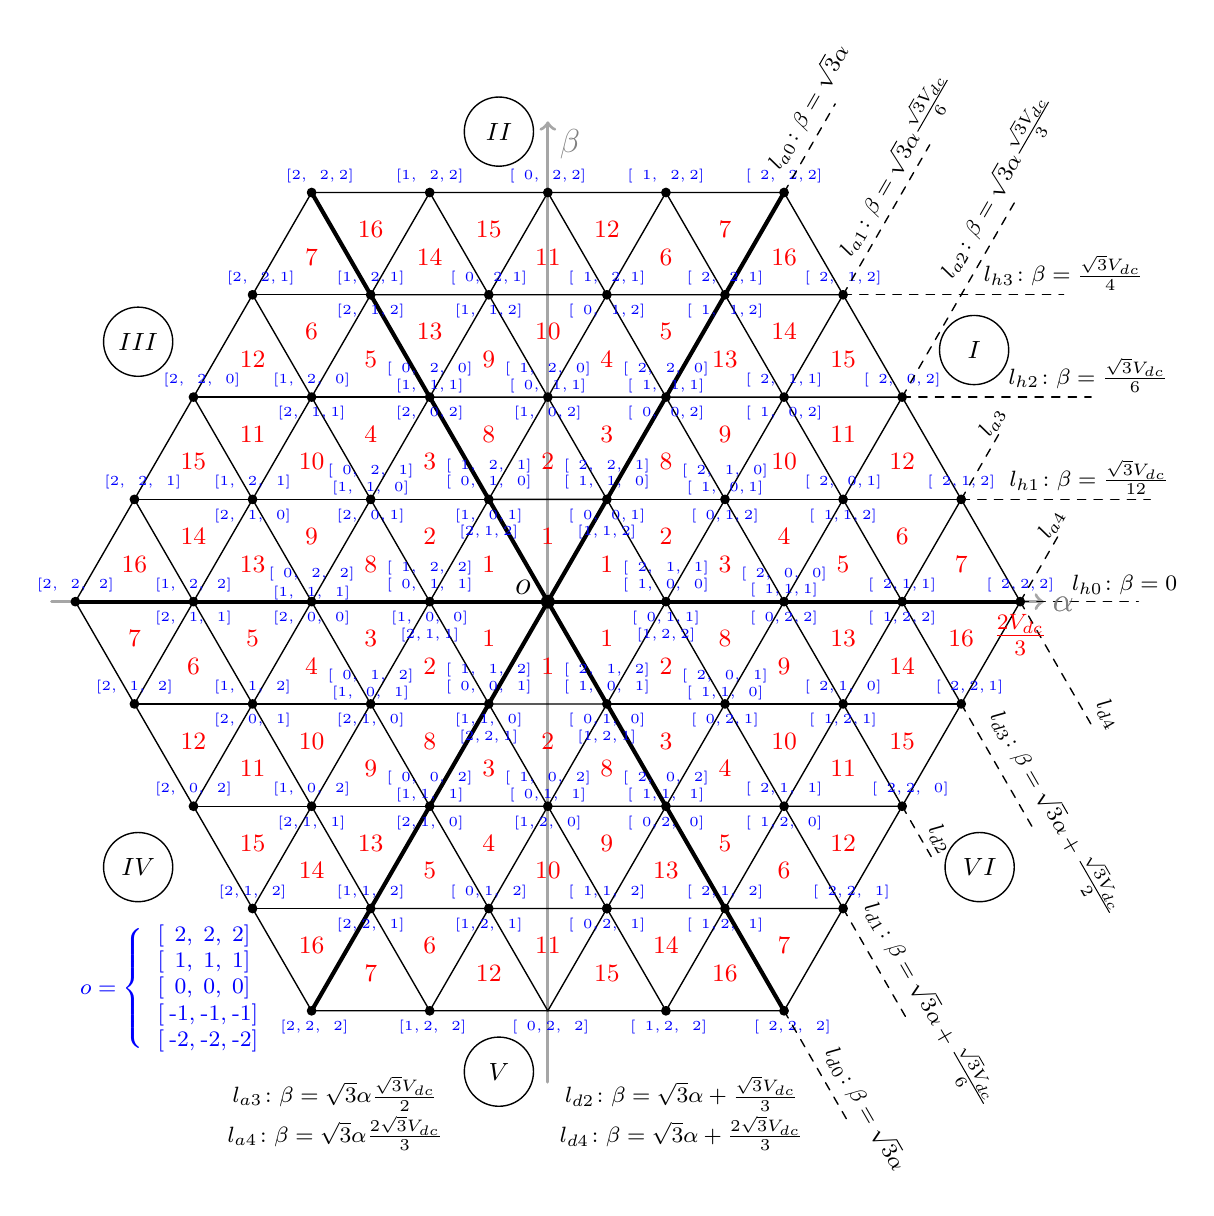
\begin{tikzpicture}

%coordinate
	\draw (0,0) coordinate [ label={ [color=black, xshift=-9, yshift=-1] \large $o$ } ] (P0);
	\draw (P0)++(\axx,0) coordinate [ label={ [color=gray, xshift=7, yshift=-7] \large $\alpha$ }] (P1){};
	\draw (P0)++(-\axx,0) coordinate (P2);
	\draw (P0)++(0,\axy) coordinate [label={[color=gray, xshift=8, yshift=-17] \large $\beta$ }] (P3) {};
	\draw (P0)++(0,-\axy) coordinate(P4);
	\draw [->, very thick, color=gray!70] (P2)--(P1);
	\draw [->, very thick, color=gray!70] (P4)--(P3);
	\filldraw [\LVcolor] (P0) circle (1.5*\fillsize pt);

%Vectors
	%Vector 4
	\draw (0,0)++ (\Vfour,0) coordinate (P2N2N2) ;
	\filldraw [\LVcolor,] (P2N2N2) circle (\fillsize pt);
	\draw (0,0)++ (60:\Vfour) coordinate (P2P2N2) ;
	\filldraw [\LVcolor] (P2P2N2) circle (\fillsize pt);
	\draw (0,0) ++ (120:\Vfour) coordinate (N2P2N2) ;
	\filldraw [\LVcolor] (N2P2N2) circle (\fillsize pt);
	\draw (0,0) ++ (-\Vfour,0) coordinate (N2P2P2);
	\filldraw [\LVcolor] (N2P2P2) circle (\fillsize pt);
	\draw (0,0)++ (240:\Vfour) coordinate (N2N2P2) ;
	\filldraw [\LVcolor] (N2N2P2) circle (\fillsize pt);
	\draw (0,0) ++ (300:\Vfour) coordinate (P2N2P2) ;
	\filldraw [\LVcolor] (P2N2P2) circle (\fillsize pt);
	%Vector 3
	\draw (0,0) ++ (\Vthree,0) coordinate (P2N1N1) ;
	\filldraw [\LVcolor] (P2N1N1) circle (\fillsize pt);
	\draw (0,0)++ (60: \Vthree) coordinate (P2P2N1) ;
	\filldraw [\LVcolor] (P2P2N1) circle (\fillsize pt);
	\draw (0,0) ++ (120: \Vthree) coordinate (N1P2N1) ;
	\filldraw [\LVcolor] (N1P2N1) circle (\fillsize pt);
	\draw (0,0) ++ (-\Vthree,0) coordinate (N1P2P2) ;
	\filldraw [\LVcolor] (N1P2P2) circle (\fillsize pt);
	\draw (0,0) ++ (240: \Vthree) coordinate (N1N1P2) ;
	\filldraw [\LVcolor] (N1N1P2) circle (\fillsize pt);
	\draw (0,0) ++ (300: \Vthree) coordinate (P2N1P2) ;
	\filldraw [\LVcolor] (P2N1P2) circle (\fillsize pt);
	%Vector 2
	\draw (0,0)++(\Vtwo,0) coordinate (P2OO) ;
	\filldraw [\LVcolor] (P2OO) circle (\fillsize pt);
	\draw (0,0) ++ (60: \Vtwo) coordinate (P2P2O) ;
	\filldraw [\LVcolor] (P2P2O) circle (\fillsize pt);
	\draw (0,0)++ (120: \Vtwo) coordinate (OP2O) ;
	\filldraw [\LVcolor] (OP2O) circle (\fillsize pt);
	\draw (0,0) ++ (-\Vtwo,0) coordinate (OP2P2) ;
	\filldraw [\LVcolor] (OP2P2) circle (\fillsize pt);
	\draw (0,0) ++ (240: \Vtwo) coordinate (OOP2) ;
	\filldraw [\LVcolor] (OOP2) circle (\fillsize pt);
	\draw (0,0) ++ (300: \Vtwo) coordinate (P2OP2) ;
	\filldraw [\LVcolor] (P2OP2) circle (\fillsize pt);
	%Vector 1
	\draw (0,0) ++ (\Vone,0) coordinate (P2P1P1) ;
	\filldraw [\LVcolor] (P2P1P1) circle (\fillsize pt);
	\draw (0,0) ++ (60:\Vone) coordinate (P2P2P1) ;
	\filldraw [\LVcolor] (P2P2P1) circle (\fillsize pt);
	\draw (0,0) ++ (120: \Vone) coordinate (P1P2P1) ;
	\filldraw [\LVcolor] (P1P2P1) circle (\fillsize pt);
	\draw (0,0) ++ (-\Vone,0) coordinate (P1P2P2) ;
	\filldraw [\LVcolor](P1P2P2) circle (\fillsize pt);
	\draw (0,0) ++ (240: \Vone) coordinate (P1P1P2) ;
	\filldraw [\LVcolor] (P1P1P2) circle (\fillsize pt);
	\draw (0,0)++ (300: \Vone) coordinate (P2P1P2) ;
	\filldraw [\LVcolor] (P2P1P2) circle (\fillsize pt);

% LINES
	%Surrounding lines
	% V4 Lines
	\draw (P2N2N2)--(P2P2N2)--(N2P2N2)--(N2P2P2)--(N2N2P2)--(P2N2P2)--(P2N2N2);
	%V3
	\draw (P2N1N1) -- (P2P2N1) -- (N1P2N1)-- (N1P2P2)-- (N1N1P2)-- (P2N1P2) --(P2N1N1) ;
	%V2 Lines 
	\draw (P2OO)-- (P2P2O)-- (OP2O) -- (OP2P2)-- (OOP2) -- (P2OP2)-- (P2OO);
	%V1 Lines 
	\draw (P2P1P1) -- (P2P2P1) --(P1P2P1)-- (P1P2P2) --(P1P1P2) --(P2P1P2)-- (P2P1P1);
	%Line inside sectors
	%SECTOR 1
	%Ascending line
	\draw (P2P1P1)++(60: \Vone) coordinate (P2P1O);
	\draw (P2P1P1) --(P2P1O);
	\filldraw [black] (P2P1O) circle (\fillsize pt);
	\draw (P2P1O)++(60: \Vone) coordinate (P2P1N1); % R11
	\draw (P2P1O) --(P2P1N1);
	\filldraw [black] (P2P1N1) circle (\fillsize pt);
	\draw (P2P1N1)++(60: \Vone) coordinate (P2P1N2);
	\draw (P2P1N1) --(P2P1N2);
	\filldraw [black] (P2P1N2) circle (\fillsize pt);
	%Descending line
	\draw (P2P1P1)++(-60: \Vone) coordinate (P2OP1);
	\draw (P2P1P1) --(P2OP1);
	\filldraw [black] (P2OP1) circle (\fillsize pt);
	\draw (P2OP1)++(-60: \Vone) coordinate (P2N1P1);
	\draw (P2OP1) --(P2N1P1);
	\filldraw [black] (P2N1P1) circle (\fillsize pt);
	\draw (P2N1P1)++(-60: \Vone) coordinate (P2N2P1);
	\draw (P2N1P1) --(P2N2P1);
	\filldraw [black] (P2N2P1) circle (\fillsize pt);
	%Direct Lines originating from [2,0,0] (P2OO)
	%Ascending line
	\draw (P2OO)++(60: \Vone) coordinate (P2ON1);% R11
	\draw (P2OO) --(P2ON1);
	\filldraw [black] (P2ON1) circle (\fillsize pt);
	\draw (P2ON1)++(60: \Vone) coordinate (P2ON2); % R11
	\draw (P2ON1) --(P2ON2);
	\filldraw [black] (P2ON2) circle (\fillsize pt);
	%Descending line
	\draw (P2OO)++(-60: \Vone) coordinate (P2N1O);
	\draw (P2OO) --(P2N1O);
	\filldraw [black] (P2N1O) circle (\fillsize pt);
	\draw (P2N1O)++(-60: \Vone) coordinate (P2N2O);
	\draw (P2N1O) --(P2N2O);
	\filldraw [black] (P2N2O) circle (\fillsize pt);
	%Direct Lines originating from [2,-1,-1] (P2N1N1)
	%Ascending line
	\draw (P2N1N1)++(60: \Vone) coordinate (P2N1N2);
	\draw (P2N1N1) --(P2N1N2);
	\filldraw [black] (P2N1N2) circle (\fillsize pt);
	%Descending line
	\draw (P2N1N1)++(-60: \Vone) coordinate (P2N2N1);
	\draw (P2N1N1) --(P2N2N1);
	\filldraw [black] (P2N2N1) circle (\fillsize pt);
	%Direct Lines originating from [2,2,1] (P2P2P1)
	%Flat line
	\draw (P2P2P1)--(P2N1N2);
	%Descending line
	\draw (P2P2P1)++(120: \Vone) coordinate (P1P2O);
	\draw (P2P2P1) --(P1P2O);
	\filldraw [black] (P1P2O) circle (\fillsize pt);
	\draw (P1P2O)++(120: \Vone) coordinate (OP2N1);
	\draw (P1P2O) --(OP2N1);
	\filldraw [black] (OP2N1) circle (\fillsize pt);
	\draw (OP2N1)++(120: \Vone) coordinate (N1P2N2);
	\draw (OP2N1) --(N1P2N2);
	\filldraw [black] (N1P2N2) circle (\fillsize pt);
	%Direct Lines originating from [2,2,0] (P2P2O)
	%Flat line
	\draw (P2P2O)--(P2ON2);
	%Descending line
	\draw (P2P2O)++(120: \Vone) coordinate (P1P2N1);
	\draw (P2P2O) --(P1P2N1);
	\filldraw [black] (P1P2N1) circle (\fillsize pt);
	\draw (P1P2N1)++(120: \Vone) coordinate (OP2N2);
	\draw (P1P2N1) --(OP2N2);
	\filldraw [black] (OP2N2) circle (\fillsize pt);
	%Direct Lines originating from [2,2,-1] (P2P2N1)
	%ASCENDING line
	\draw (P2P2N1)--(P2P1N2);
	%Descending line
	\draw (P2P2N1)++(120: \Vone) coordinate (P1P2N2);
	\draw (P2P2N1) --(P1P2N2);
	\filldraw [black] (P1P2N2) circle (\fillsize pt);
	
	%SECTOR 2
	%Direct Lines originating from [1,2,1] (P1P2P1)
	%Ascending line
	\draw (P1P2P1) --(P1P2N2);
	%Flat line
	\draw (P1P2P1)++(-\Vone, 0) coordinate (OP2P1);
	\filldraw [black] (OP2P1) circle (\fillsize pt);
	\draw (P1P2P1)++(-2* \Vone, 0) coordinate (N1P2P1); % 
	\filldraw [black] (N1P2P1) circle (\fillsize pt);
	\draw (P1P2P1)++(-3* \Vone, 0) coordinate (N2P2P1);
	\filldraw [black] (N2P2P1) circle (\fillsize pt);
	\draw (P1P2P1) -- (N2P2P1);
	%Direct Lines originating from [0,2,0] (OP2O)
	%Ascending line
	\draw (OP2O) --(OP2N2);
	%Flat line
	\draw (OP2O)++(-\Vone, 0) coordinate (N1P2O);
	\filldraw [black] (N1P2O) circle (\fillsize pt);
	\draw (OP2O)++(-2* \Vone, 0) coordinate (N2P2O);
	\filldraw [black] (N2P2O) circle (\fillsize pt);
	\draw (OP2O) -- (N2P2O);
	%Direct Lines originating from [-1,2,-1] (N1P2N1)
	%Ascending line
	\draw (N1P2N1) --(N1P2N2);
	%Flat line
	\draw (N1P2N1)++(-\Vone, 0) coordinate (N2P2N1);
	\filldraw [black] (N2P2N1) circle (\fillsize pt);
	\draw (N1P2N1) --(N2P2N1);
	%SECTOR3
	%Direct Lines originating from [1,2,2] (P1P2P1)
	%Descending line
	\draw (P1P2P2) --(N2P2N1);
	%Ascending lines
	\draw (P1P2P2)++(-120: \Vone) coordinate (OP1P2);
	\filldraw [black] (OP1P2) circle (\fillsize pt);
	\draw (P1P2P2)++(-120:2* \Vone) coordinate (N1OP2);
	\filldraw [black] (N1OP2) circle (\fillsize pt);
	\draw (P1P2P2)++(-120:3* \Vone) coordinate (N2N1P2);
	\filldraw [black] (N2N1P2) circle (\fillsize pt);
	\draw (P1P2P2) --(N2N1P2);
	%Direct Lines originating from [0,2,2] (OP2P2)
	%Descending line
	\draw (OP2P2) --(N2P2O);
	%Ascending lines
	\draw (OP2P2)++(-120: \Vone) coordinate (N1P1P2);
	\filldraw [black] (N1P1P2) circle (\fillsize pt);
	\draw (OP2P2)++(-120: 2* \Vone) coordinate (N2OP2);
	\filldraw [black] (N2OP2) circle (\fillsize pt);
	\draw (OP2P2) -- (N2OP2);
	%Direct Lines originating from [-1,2,2] (N1P2P2)
	%Descending line
	\draw (N1P2P2)--(N2P2P1); 
	%Ascending line
	\draw (N1P2P2)++(-120: \Vone) coordinate (N2P1P2);
	\draw (N1P2P2) --(N2P1P2);
	\filldraw [black] (N2P1P2) circle (\fillsize pt);
	%
	%SECTOR4
	%Direct Lines originating from [1,1,2] (P1P1P2)
	%flat line(s)
	\draw (P1P1P2) --(N2P1P2);
	% descending line(s)
	\draw (P1P1P2)++(-60: \Vone) coordinate (P1OP2);
	\filldraw [black] (P1OP2) circle (\fillsize pt);
	\draw (P1P1P2)++(-60: 2*\Vone) coordinate (P1N1P2);
	\filldraw [black] (P1N1P2) circle (\fillsize pt);
	\draw (P1P1P2)++(-60: 3*\Vone) coordinate (P1N2P2);
	\filldraw [black] (P1N2P2) circle (\fillsize pt);
	\draw (P1P1P2) --(P1N2P2);
	%Direct Lines originating from [0,0,2] (OOP2)
	%flat line(s)
	\draw (OOP2) --(N2OP2);
	% descending line(s)
	\draw (OOP2)++(-60: \Vone) coordinate (ON1P2);
	\filldraw [black] (ON1P2) circle (\fillsize pt);
	\draw (OOP2)++(-60: 2*\Vone) coordinate (ON2P2);
	\filldraw [black] (P1N1P2) circle (\fillsize pt);
	\draw (OOP2) --(ON2P2);
	%Direct Lines originating from [-1,-1,2] (N1N1P2)
	%flat line(s)
	\draw (N1N1P2) --(N2N1P2);
	% descending line(s)
	\draw (N1N1P2)++(-60: \Vone) coordinate (N1N2P2);
	\filldraw [black] (N1N2P2) circle (\fillsize pt);
	\draw (N1N1P2) --(N1N2P2);
	%SECTOR5
	%Direct Lines originating from [2,1,2] (P2P1P2)
	%flat line(s)
	\draw (P2P1P2) --(P2N2N1);
	%ascending line(s)
	\draw (P2P1P2) --(N1N2P2);
	%Direct Lines originating from [2,0,2] (P2OP2)
	%flat line(s)
	\draw (P2OP2) --(P2N2O);
	%ascending line(s)
	\draw (P2OP2) --(ON2P2);
	%Direct Lines originating from [2,-1,2] (P2N1P2)
	%flat line(s)
	\draw (P2N1P2) --(P2N2P1);
	%ascending line(s)
	\draw (P2N1P2) --(P1N2P2);
	%% bold lines for sectors
	\draw [\LVcolor, line width=\LVwdt pt] (P0)--(P2N2N2);
	\draw [\LVcolor, line width=\LVwdt pt] (P0)--(P2P2N2);
	\draw [\LVcolor, line width=\LVwdt pt] (P0)--(N2P2N2);
	\draw [\LVcolor, line width=\LVwdt pt ](P0)--(N2P2P2);
	\draw [\LVcolor, line width=\LVwdt pt ] (P0)--(N2N2P2);
	\draw [\LVcolor, line width=\LVwdt pt] (P0)--(P2N2P2);
%DESCRIPTIONS
	%Outer Hexagon
	% 0 degree
	\coordinate [label={[\Vnamecolor, xshift=0, yshift=0] \tiny $[\:\:2,\shortminus2,\shortminus2]$ }] (P2N2N2) at (P2N2N2);
	% 15 degree
	\coordinate [label={[\Vnamecolor, xshift=0, yshift=0] \tiny $[\:\:2,\shortminus1,\shortminus2]$ }] (P2N1N2) at (P2N1N2);
	% 30 degree
	\coordinate [label={[\Vnamecolor, xshift=0, yshift=0] \tiny $[\:\:2,\:\:0,\shortminus2]$ }] (P2ON2) at (P2ON2);
	%45 degree
	\coordinate [label={[\Vnamecolor, xshift=0, yshift=0] \tiny $[\:\:2,\:\:1,\shortminus2]$ }] (P2P1N2) at (P2P1N2);
	%60 degree
	\coordinate [label={[\Vnamecolor, xshift=0, yshift=0] \tiny $[\:\:2,\:\:2,\shortminus2]$ }] (P2P2N2) at (P2P2N2);
	%75 degree
	\coordinate [label={[\Vnamecolor, xshift=0, yshift=0] \tiny $[\:\:1,\:\:2,\shortminus2]$ }] (P1P2N2) at (P1P2N2);
	%90 degree
	\coordinate [label={[\Vnamecolor, xshift=0, yshift=0] \tiny $[\:\:0,\:\:2,\shortminus2]$ }] (OP2N2) at (OP2N2);
	%105 degree
	\coordinate [label={[\Vnamecolor, xshift=0, yshift=0] \tiny $[\shortminus1,\:\:2,\shortminus2]$ }] (N1P2N2) at (N1P2N2);
	%120 degree
	\coordinate [label={[\Vnamecolor, xshift=3, yshift=0] \tiny $[\shortminus2,\:\:2,\shortminus2]$ }] (N2P2N2) at (N2P2N2);
	%135 degree
	\coordinate [label={[\Vnamecolor, xshift=3, yshift=0] \tiny $[\shortminus2,\:\:2,\shortminus1]$ }] (N2P2N1) at (N2P2N1);
	%150 degree
	\coordinate [label={[\Vnamecolor, xshift=3, yshift=0] \tiny $[\shortminus2,\:\:2,\:\:0]$ }] (N2P2O) at (N2P2O);
	%165 degree
	\coordinate [label={[\Vnamecolor, xshift=3, yshift=0] \tiny $[\shortminus2,\:\:2,\:\:1]$ }] (N2P2P1) at (N2P2P1);
	%180 degree
	\coordinate [label={[\Vnamecolor, xshift=0, yshift=0] \tiny $[\shortminus2,\:\:2,\:\:2]$ }] (N2P2P2) at (N2P2P2);
	%195 degree
	\coordinate [label={[\Vnamecolor, xshift=0, yshift=0] \tiny $[\shortminus2,\:\:1,\:\:2]$ }] (N2P1P2) at (N2P1P2);
	%210 degree
	\coordinate [label={[\Vnamecolor, xshift=0, yshift=0] \tiny $[\shortminus2,\:\:0,\:\:2]$ }] (N2OP2) at (N2OP2);
	%225 degree
	\coordinate [label={[\Vnamecolor, xshift=0, yshift=0] \tiny $[\shortminus2,\shortminus1,\:\:2]$ }] (N2N1P2) at (N2N1P2);
	%240 degree
	\coordinate [label={[\Vnamecolor, xshift=1, yshift=-12] \tiny $[\shortminus2,\shortminus2,\:\:2]$ }] (N2N2P2) at (N2N2P2);
	%255 degree
	\coordinate [label={[\Vnamecolor, xshift=1, yshift=-12] \tiny $[\shortminus1,\shortminus2,\:\:2]$ }] (N1N2P2) at (N1N2P2);
	%270 degree
	\coordinate [label={[\Vnamecolor, xshift=1, yshift=-12] \tiny $[\:\:0,\shortminus2,\:\:2]$ }] (ON2P2) at (ON2P2);
	%285 degree
	\coordinate [label={[\Vnamecolor, xshift=1, yshift=-12] \tiny $[\:\:1,\shortminus2,\:\:2]$ }] (P1N2P2) at (P1N2P2);
	%300 degree
	\coordinate [label={[\Vnamecolor, xshift=3, yshift=-12] \tiny $[\:\:2,\shortminus2,\:\:2]$ }] (P2N2P2) at (P2N2P2);
	%315 degree
	\coordinate [label={[\Vnamecolor, xshift=3, yshift=0] \tiny $[\:\:2,\shortminus2,\:\:1]$ }] (P2N2P1) at (P2N2P1);
	%330 degree
	\coordinate [label={[\Vnamecolor, xshift=3, yshift=0] \tiny $[\:\:2,\shortminus2,\:\:0]$ }] (P2N2O) at (P2N2O);
	%345degree
	\coordinate [label={[\Vnamecolor, xshift=3, yshift=0] \tiny $[\:\:2,\shortminus2,\shortminus1]$ }] (P2N2N1) at (P2N2N1);
	%Third Hexagon
	% 0 degree
	\coordinate [label={[\Vnamecolor, xshift=0, yshift=0] \tiny $[\:\:2,\shortminus1,\shortminus1]$ }] (P2N1N1) at (P2N1N1);
	\coordinate [label={[\Vnamecolor, xshift=0, yshift=-12] \tiny $[\:\:1,\shortminus2,\shortminus2]$ }] (P2N1N1) at (P2N1N1);
	%20 degree
	\coordinate [label={[\Vnamecolor, xshift=0, yshift=0] \tiny $[\:\:2,\:\:0,\shortminus1]$ }] (P2ON1) at (P2ON1);
	\coordinate [label={[\Vnamecolor, xshift=0, yshift=-12] \tiny $[\:\:1,\shortminus1,\shortminus2]$ }] (P2ON1) at (P2ON1);
	%40 degree
	\coordinate [label={[\Vnamecolor, xshift=0, yshift=0] \tiny $[\:\:2,\:\:1,\shortminus1]$ }] (P2P1N1) at (P2P1N1);
	\coordinate [label={[\Vnamecolor, xshift=0, yshift=-12] \tiny $[\:\:1,\:\:0,\shortminus2]$ }](P2P1N1) at (P2P1N1);
	%60 degree
	\coordinate [label={[\Vnamecolor, xshift=0, yshift=0] \tiny $[\:\:2,\:\:2,\shortminus1]$ }] (P2P2N1) at (P2P2N1);
	\coordinate [label={[\Vnamecolor, xshift=0, yshift=-12] \tiny $[\:\:1,\:\:1,\shortminus2]$ }] (P2P2N1) at (P2P2N1);
	%80 degree
	\coordinate [label={[\Vnamecolor, xshift=0, yshift=0] \tiny $[\:\:1,\:\:2,\shortminus1]$ }] (P1P2N1) at (P1P2N1);
	\coordinate [label={[\Vnamecolor, xshift=0, yshift=-12] \tiny $[\:\:0,\:\:1,\shortminus2]$ }] (P1P2N1) at (P1P2N1);
	%100 degree
	\coordinate [label={[\Vnamecolor, xshift=0, yshift=0] \tiny $[\:\:0,\:\:2,\shortminus1]$ }] (OP2N1) at (OP2N1);
	\coordinate [label={[\Vnamecolor, xshift=0, yshift=-12] \tiny $[\shortminus1,\:\:1,\shortminus2]$ }] (OP2N1) at (OP2N1);
	%120 degree
	\coordinate [label={[\Vnamecolor, xshift=0, yshift=0] \tiny $[\shortminus1,\:\:2,\shortminus1]$ }] (N1P2N1) at (N1P2N1);
	\coordinate [label={[\Vnamecolor, xshift=0, yshift=-12] \tiny $[\shortminus2,\:\:1,\shortminus2]$ }] (N1P2N1) at (N1P2N1);
	%140 degree
	\coordinate [label={[\Vnamecolor, xshift=0, yshift=0] \tiny $[\shortminus1,\:\:2,\:\:0]$ }] (N1P2O) at (N1P2O);
	\coordinate [label={[\Vnamecolor, xshift=0, yshift=-12] \tiny $[\shortminus2,\:\:1,\shortminus1]$ }] (N1P2O) at (N1P2O);
	%160 degree
	\coordinate [label={[\Vnamecolor, xshift=0, yshift=0] \tiny $[\shortminus1,\:\:2,\:\:1]$ }] (N1P2P1) at (N1P2P1);
	\coordinate [label={[\Vnamecolor, xshift=0, yshift=-12] \tiny $[\shortminus2,\:\:1,\:\:0]$ }] (N1P2P1) at (N1P2P1);
	%180 degree
	\coordinate [label={[\Vnamecolor, xshift=0, yshift=0] \tiny $[\shortminus1,\:\:2,\:\:2]$ }] (N1P2P2) at (N1P2P2);
	\coordinate [label={[\Vnamecolor, xshift=0, yshift=-12] \tiny $[\shortminus2,\:\:1,\:\:1]$ }] (N1P2P2) at (N1P2P2);
	%200 degree
	\coordinate [label={[\Vnamecolor, xshift=0, yshift=0] \tiny $[\shortminus1,\:\:1,\:\:2]$ }] (N1P1P2) at (N1P1P2);
	\coordinate [label={[\Vnamecolor, xshift=0, yshift=-12] \tiny $[\shortminus2,\:\:0,\:\:1]$ }] (N1P1P2) at (N1P1P2);
	%220 degree
	\coordinate [label={[\Vnamecolor, xshift=0, yshift=0] \tiny $[\shortminus1,\:\:0,\:\:2]$ }] (N1OP2) at (N1OP2);
	\coordinate [label={[\Vnamecolor, xshift=0, yshift=-12] \tiny $[\shortminus2,\shortminus1,\:\:1]$ }] (N1OP2) at (N1OP2);
	%240 degree
	\coordinate [label={[\Vnamecolor, xshift=0, yshift=0] \tiny $[\shortminus1,\shortminus1,\:\:2]$ }] (N1N1P2) at (N1N1P2);
	\coordinate [label={[\Vnamecolor, xshift=0, yshift=-12] \tiny $[\shortminus2,\shortminus2,\:\:1]$ }] (N1N1P2) at (N1N1P2);
	%260 degree
	\coordinate [label={[\Vnamecolor, xshift=0, yshift=0] \tiny $[\:\:0,\shortminus1,\:\:2]$ }] (ON1P2) at (ON1P2);
	\coordinate [label={[\Vnamecolor, xshift=0, yshift=-12] \tiny $[\shortminus1,\shortminus2,\:\:1]$ }] (ON1P2) at (ON1P2);
	%280 degree
	\coordinate [label={[\Vnamecolor, xshift=0, yshift=0] \tiny $[\:\:1,\shortminus1,\:\:2]$ }] (P1N1P2) at (P1N1P2);
	\coordinate [label={[\Vnamecolor, xshift=0, yshift=-12] \tiny $[\:\:0,\shortminus2,\:\:1]$ }] (P1N1P2) at (P1N1P2);
	%300 degree
	\coordinate [label={[\Vnamecolor, xshift=0, yshift=0] \tiny $[\:\:2,\shortminus1,\:\:2]$ }] (P2N1P2) at (P2N1P2);
	\coordinate [label={[\Vnamecolor, xshift=0, yshift=-12] \tiny $[\:\:1,\shortminus2,\:\:1]$ }] (P2N1P2) at (P2N1P2);
	%320 degree
	\coordinate [label={[\Vnamecolor, xshift=0, yshift=0] \tiny $[\:\:2,\shortminus1,\:\:1]$ }] (P2N1P1) at (P2N1P1);
	\coordinate [label={[\Vnamecolor, xshift=0, yshift=-12] \tiny $[\:\:1,\shortminus2,\:\:0]$ }] (P2N1P1) at (P2N1P1);
	%340 degree
	\coordinate [label={[\Vnamecolor, xshift=0, yshift=0] \tiny $[\:\:2,\shortminus1,\:\:0]$ }] (P2N1O) at (P2N1O);
	\coordinate [label={[\Vnamecolor, xshift=0, yshift=-12] \tiny $[\:\:1,\shortminus2,\shortminus1]$ }] (P2N1O) at (P2N1O);
	%Second Hexagon
	% 0 degree
	\coordinate [label={[\Vnamecolor, xshift=0, yshift=4] \tiny $[\:\:2,\:\:0,\:\:0]$ }] (P2OO) at (P2OO);
	\coordinate [label={[\Vnamecolor, xshift=0, yshift=-2] \tiny $[\:\:1,\shortminus1,\shortminus1]$ }] (P2OO) at (P2OO);
	\coordinate [label={[\Vnamecolor, xshift=0, yshift=-12] \tiny $[\:\:0,\shortminus2,\shortminus2]$ }] (P2OO) at (P2OO);
	% 30 degree
	\coordinate [label={[\Vnamecolor, xshift=0, yshift=4] \tiny $[\:\:2,\:\:1,\:\:0]$ }] (P2P1O) at (P2P1O);
	\coordinate [label={[\Vnamecolor, xshift=0, yshift=-2] \tiny $[\:\:1,\:\:0,\shortminus1]$ }] (P2P1O) at (P2P1O);
	\coordinate [label={[\Vnamecolor, xshift=0, yshift=-12] \tiny $[\:\:0,\shortminus1,\shortminus2]$ }] (P2P1O) at (P2P1O);
	% 60 degree
	\coordinate [label={[\Vnamecolor, xshift=0, yshift=4] \tiny $[\:\:2,\:\:2,\:\:0]$ }] (P2P2O) at (P2P2O);
	\coordinate [label={[\Vnamecolor, xshift=0, yshift=-2] \tiny $[\:\:1,\:\:1,\shortminus1]$ }] (P2P2O) at (P2P2O);
	\coordinate [label={[\Vnamecolor, xshift=0, yshift=-12] \tiny $[\:\:0,\:\:0,\shortminus2]$ }] (P2P2O) at (P2P2O);
	% 90 degree
	\coordinate [label={[\Vnamecolor, xshift=0, yshift=4] \tiny $[\:\:1,\:\:2,\:\:0]$ }] (P1P2O) at (P1P2O);
	\coordinate [label={[\Vnamecolor, xshift=0, yshift=-2] \tiny $[\:\:0,\:\:1,\shortminus1]$ }] (P1P2O) at (P1P2O);
	\coordinate [label={[\Vnamecolor, xshift=0, yshift=-12] \tiny $[\shortminus1,\:\:0,\shortminus2]$ }] (P1P2O) at (P1P2O);
	% 120 degree
	\coordinate [label={[\Vnamecolor, xshift=0, yshift=4] \tiny $[\:\:0,\:\:2,\:\:0]$ }] (OP2O) at (OP2O) ;
	\coordinate [label={[\Vnamecolor, xshift=0, yshift=-2] \tiny $[\shortminus1,\:\:1,\shortminus1]$ }] (OP2O) at (OP2O) ;
	\coordinate [label={[\Vnamecolor, xshift=0, yshift=-12] \tiny $[\shortminus2,\:\:0,\shortminus2]$ }] (OP2O) at (OP2O) ;
	% 150 degree
	\coordinate [label={[\Vnamecolor, xshift=0, yshift=4] \tiny $[\:\:0,\:\:2,\:\:1]$ }] (OP2P1) at (OP2P1) ;
	\coordinate [label={[\Vnamecolor, xshift=0, yshift=-2] \tiny $[\shortminus1,\:\:1,\:\:0]$ }] (OP2P1) at (OP2P1) ;
	\coordinate [label={[\Vnamecolor, xshift=0, yshift=-12] \tiny $[\shortminus2,\:\:0,\shortminus1]$ }] (OP2P1) at (OP2P1) ;
	% 180 degree
	\coordinate [label={[\Vnamecolor, xshift=0, yshift=4] \tiny $[\:\:0,\:\:2,\:\:2]$ }] (OP2P2) at (OP2P2);
	\coordinate [label={[\Vnamecolor, xshift=0, yshift=-3] \tiny $[\shortminus1,\:\:1,\:\:1]$ }] (OP2P2) at (OP2P2) ;
	\coordinate [label={[\Vnamecolor, xshift=0, yshift=-12] \tiny $[\shortminus2,\:\:0,\:\:0]$ }] (OP2P2) at (OP2P2) ;
	% 210 degree
	\coordinate [label={[\Vnamecolor, xshift=0, yshift=4] \tiny $[\:\:0,\:\:1,\:\:2]$ }] (OP1P2) at (OP1P2);
	\coordinate [label={[\Vnamecolor, xshift=0, yshift=-2] \tiny $[\shortminus1,\:\:0,\:\:1]$ }] (OP1P2) at (OP1P2);
	\coordinate [label={[\Vnamecolor, xshift=0, yshift=-12] \tiny $[\shortminus2,\shortminus1,\:\:0]$ }] (OP1P2) at (OP1P2);
	% 240 degree
	\coordinate [label={[\Vnamecolor, xshift=0, yshift=4] \tiny $[\:\:0,\:\:0,\:\:2]$ }] (OOP2) at (OOP2) ;
	\coordinate [label={[\Vnamecolor, xshift=0, yshift=-2] \tiny $[\shortminus1,\shortminus1,\:\:1]$ }] (OOP2) at (OOP2) ;
	\coordinate [label={[\Vnamecolor, xshift=0, yshift=-12] \tiny $[\shortminus2,\shortminus1,\:\:0]$ }] (OOP2) at (OOP2) ;
	% 270 degree
	\coordinate [label={[\Vnamecolor, xshift=0, yshift=4] \tiny $[\:\:1,\:\:0,\:\:2]$ }] (P1OP2) at (P1OP2);
	\coordinate [label={[\Vnamecolor, xshift=0, yshift=-2] \tiny $[\:\:0,\shortminus1,\:\:1]$ }] (P1OP2) at (P1OP2);
	\coordinate [label={[\Vnamecolor, xshift=0, yshift=-12] \tiny $[\shortminus1,\shortminus2,\:\:0]$ }] (P1OP2) at (P1OP2);
	% 300 degree
	\coordinate [label={[\Vnamecolor, xshift=0, yshift=4] \tiny $[\:\:2,\:\:0,\:\:2]$ }] (P2OP2) at (P2OP2) ;
	\coordinate [label={[\Vnamecolor, xshift=0, yshift=-2] \tiny $[\:\:1,\shortminus1,\:\:1]$ }] (P2OP2) at (P2OP2) ;
	\coordinate [label={[\Vnamecolor, xshift=0, yshift=-12] \tiny $[\:\:0,\shortminus2,\:\:0]$ }] (P2OP2) at (P2OP2) ;
	% 330 degree
	\coordinate [label={[\Vnamecolor, xshift=0, yshift=4] \tiny $[\:\:2,\:\:0,\:\:1]$ }] (P2OP1) at (P2OP1);
	\coordinate [label={[\Vnamecolor, xshift=0, yshift=-2] \tiny $[\:\:1,\shortminus1,\:\:0]$ }] (P2OP1) at (P2OP1);
	\coordinate [label={[\Vnamecolor, xshift=0, yshift=-12] \tiny $[\:\:0,\shortminus2,\shortminus1]$ }] (P2OP1) at (P2OP1);
	% First Hexagon
	% 0 degree
	\coordinate [label={[\Vnamecolor, xshift=0, yshift=6] \tiny $[\:\:2,\:\:1,\:\:1]$ }] (P2P1P1) at (P2P1P1);
	\coordinate [label={[\Vnamecolor, xshift=0, yshift=0] \tiny $[\:\:1,\:\:0,\:\:0]$ }] (P2P1P1) at (P2P1P1);
	\coordinate [label={[\Vnamecolor, xshift=0, yshift=-12] \tiny $[\:\:0,\shortminus1,\shortminus1]$ }] (P2P1P1) at (P2P1P1);
	\coordinate [label={[\Vnamecolor, xshift=0, yshift=-18] \tiny $[\shortminus1,\shortminus2,\shortminus2]$ }] (P2P1P1) at (P2P1P1);
	% 60 degree
	\coordinate [label={[\Vnamecolor, xshift=0, yshift=6] \tiny $[\:\:2,\:\:2,\:\:1]$ }] (P2P2P1) at (P2P2P1);
	\coordinate [label={[\Vnamecolor, xshift=0, yshift=0] \tiny $[\:\:1,\:\:1,\:\:0]$ }] (P2P2P1)at (P2P2P1) ;
	\coordinate [label={[\Vnamecolor, xshift=0, yshift=-12] \tiny $[\:\:0,\:\:0,\shortminus1]$ }] (P2P2P1)at (P2P2P1) ;
	\coordinate [label={[\Vnamecolor, xshift=0, yshift=-18] \tiny $[\shortminus1,\shortminus1,\shortminus2]$ }] (P2P2P1) at (P2P2P1);
	% 120 degree
	\coordinate [label={[\Vnamecolor, xshift=0, yshift=6] \tiny $[\:\:1,\:\:2,\:\:1]$ }] (P1P2P1) at (P1P2P1);
	\coordinate [label={[\Vnamecolor, xshift=0, yshift=0] \tiny $[\:\:0,\:\:1,\:\:0]$ }] (P1P2P1) at (P1P2P1) ;
	\coordinate [label={[\Vnamecolor, xshift=0, yshift=-12] \tiny $[\shortminus1,\:\:0,\shortminus1]$ }] (P1P2P1) at (P1P2P1) ;
	\coordinate [label={[\Vnamecolor, xshift=0, yshift=-18] \tiny $[\shortminus2,\shortminus1,\shortminus2]$ }] (P1P2P1) at (P1P2P1);
	% 180 degree
	\coordinate [label={[\Vnamecolor, xshift=0, yshift=6] \tiny $[\:\:1,\:\:2,\:\:2]$ }] (P1P2P2) at (P1P2P2);
	\coordinate [label={[\Vnamecolor, xshift=0, yshift=0] \tiny $[\:\:0,\:\:1,\:\:1]$ }] (P1P2P2) at (P1P2P2);
	\coordinate [label={[\Vnamecolor, xshift=0, yshift=-12] \tiny $[\shortminus1,\:\:0,\:\:0]$ }] (P1P2P2) at (P1P2P2);
	\coordinate [label={[\Vnamecolor, xshift=0, yshift=-18] \tiny $[\shortminus2,\shortminus1,\shortminus1]$ }] (P1P2P2) at (P1P2P2);
	% 240 degree
	\coordinate [label={[\Vnamecolor, xshift=0, yshift=6] \tiny $[\:\:1,\:\:1,\:\:2]$ }] (P1P1P2) at (P1P1P2);
	\coordinate [label={[\Vnamecolor, xshift=0, yshift=0] \tiny $[\:\:0,\:\:0,\:\:1]$ }] (P1P1P2) at (P1P1P2);
	\coordinate [label={[\Vnamecolor, xshift=0, yshift=-12] \tiny $[\shortminus1,\shortminus1,\:\:0]$ }] (P1P1P2) at (P1P1P2);
	\coordinate [label={[\Vnamecolor, xshift=0, yshift=-18] \tiny $[\shortminus2,\shortminus2,\shortminus1]$ }] (P1P1P2) at (P1P1P2);
	% 300 degree
	\draw (0,0)++ (300: \Vone) coordinate [label={[\Vnamecolor, xshift=0, yshift=6] \tiny $[\:\:2,\:\:1,\:\:2]$ }] (P2P1P2) ;
	\draw (0,0)++ (300: \Vone) coordinate [label={[\Vnamecolor, xshift=0, yshift=0] \tiny $[\:\:1,\:\:0,\:\:1]$ }] (P2P1P2) ;
	\draw (0,0)++ (300: \Vone) coordinate [label={[\Vnamecolor, xshift=0, yshift=-12] \tiny $[\:\:0,\shortminus1,\:\:0]$ }] (P2P1P2) ;
	\draw (0,0)++ (300: \Vone) coordinate [label={[\Vnamecolor, xshift=0, yshift=-18] \tiny $[\shortminus1,\shortminus2,\shortminus1]$ }] (P2P1P2) ;
	 %Zero Vector
	\filldraw [black] (P0) circle (\fillsize pt);
	\node (OOO) at (-4.7, -6) [ label={[\Vnamecolor, align=left] \footnotesize $ o=\left\{ \begin{array}{ll} $[\:\:2,\:\:2,\:\:2]$ \\ $[\:\:1,\:\:1,\:\:1]$ \\ $[\:\:0,\:\:0,\:\:0]$ \\ $[\:-1,\:-1,\:-1]$ \\ $[\:-2,\:-2,\:-2]$ \end{array} \right. $} ] {};
%Sector numbers
	\node [ xshift=26, yshift=17, circle,draw, minimum size =25] (SEC1) at (P2ON2) { $I$};
	\node [ xshift=25, yshift=22, circle,draw, minimum size =25] (SEC2) at (N1P2N2) {$II$};%%
	\node [ xshift=-20, yshift=20, circle,draw, minimum size =25] (SEC3) at (N2P2O) { $III$};
	\node [ xshift=-20, yshift=-22, circle,draw, minimum size =25] (SEC4) at (N2OP2) {$IV$};
	\node [ xshift=25, yshift=-22, circle,draw,minimum size =25] (SEC5) at (N1N2P2) {$V$};%%
	\node [ xshift=28, yshift=-22, circle,draw, minimum size =25] (SEC6) at (P2N2O) { $VI$};
%Region numbers
	%Sector 1
	\coordinate [label={[\Rnamecolor, xshift=\Xone, yshift=\Yone] $1$ }] (S1-1) at (P0); %R1
	\coordinate [label={[\Rnamecolor, xshift=0, yshift=\Ytwo] $2$ }] (S1-2) at (P2P1P1); %R2
	\coordinate [label={[\Rnamecolor,xshift=\Xone , yshift=\Yone] $3$ }] (S1-3) at (P2P1P1); %R3
	\coordinate [label={[\Rnamecolor, xshift=0, yshift=\Ytwo] $4$ }] (S1-4) at (P2OO); %R4
	\coordinate [label={[\Rnamecolor, xshift=\Xone, yshift=\Yone] $5$ }] (S1-5) at (P2OO); %R5
	\coordinate [label={[\Rnamecolor, xshift=0, yshift=\Ytwo] $6$ }] (S1-6) at (P2N1N1); %R6
	\coordinate [label={[\Rnamecolor, xshift=\Xone, yshift=\Yone] $7$ }] (S1-7) at (P2N1N1); %R7
	\coordinate [label={[\Rnamecolor, xshift=\Xone, yshift=\Yone] $8$ }] (S1-8) at (P2P2P1); %R8
	\coordinate [label={[\Rnamecolor, xshift=0, yshift=\Ytwo] $9$ }] (S1-9) at (P2P1O); %R9
	\coordinate [label={[\Rnamecolor, xshift=\Xone, yshift=\Yone] $10$ }] (S1-10) at (P2P1O); %R10
	\coordinate [label={[\Rnamecolor, xshift=0, yshift=\Ytwo] $11$ }] (S1-11) at (P2ON1); %R11
	\coordinate [label={[\Rnamecolor, xshift=\Xone, yshift=\Yone] $12$ }] (S1-12) at (P2ON1); %R12
	\coordinate [label={[\Rnamecolor, xshift=\Xone, yshift=\Yone] $13$ }] (S1-13) at (P2P2O); %R13
	\coordinate [label={[\Rnamecolor, xshift=0, yshift=\Ytwo] $14$ }] (S1-14) at (P2P1N1); %R14
	\coordinate [label={[\Rnamecolor, xshift=\Xone, yshift=\Yone] $15$ }] (S1-15) at (P2P1N1); %R15
	\coordinate [label={[\Rnamecolor, xshift=\Xone, yshift=\Yone] $16$ }] (S1-16) at (P2P2N1); %R16
	%Sector 2
	\coordinate [label={[\Rnamecolor, xshift=0, yshift=\Ytwo] $1$ }] (S2-1) at (P0); %R1
	\coordinate [label={[\Rnamecolor, xshift=\Xone, yshift=\Yone] $2$ }] (S2-2) at (P1P2P1); %R2
	\coordinate [label={[\Rnamecolor, xshift=0, yshift=\Ytwo] $3$ }] (S2-3) at (P2P2P1); %R3
	\coordinate [label={[\Rnamecolor, xshift=\Xone, yshift=\Yone] $4$ }] (S2-4) at (P1P2O); %R4
	\coordinate [label={[\Rnamecolor, xshift=0, yshift=\Ytwo] $5$ }] (S2-5) at (P2P2O); %R5
	\coordinate [label={[\Rnamecolor, xshift=\Xone, yshift=\Yone] $6$ }] (S2-6) at (P1P2N1); %R6
	\coordinate [label={[\Rnamecolor, xshift=0, yshift=\Ytwo] $7$ }] (S2-7) at (P2P2N1); %R7
	\coordinate [label={[\Rnamecolor, xshift=0, yshift=\Ytwo] $8$ }] (S2-8) at (P1P2P1); %R8
	\coordinate [label={[\Rnamecolor, xshift=\Xone, yshift=\Yone] $9$ }] (S2-9) at (OP2O); %R9
	\coordinate [label={[\Rnamecolor, xshift=0, yshift=\Ytwo] $10$ }] (S2-10) at (P1P2O); %R10
	\coordinate [label={[\Rnamecolor, xshift=\Xone, yshift=\Yone] $11$ }] (S2-11) at (OP2N1); %R11
	\coordinate [label={[\Rnamecolor, xshift=0, yshift=\Ytwo] $12$ }] (S2-12) at (P1P2N1); %R12
	\coordinate [label={[\Rnamecolor, xshift=0, yshift=\Ytwo] $13$ }] (S2-13) at (OP2O); %R13
	\coordinate [label={[\Rnamecolor, xshift=\Xone, yshift=\Yone] $14$ }] (S2-14) at (N1P2N1); %R14
	\coordinate [label={[\Rnamecolor, xshift=0, yshift=\Ytwo] $15$ }] (S2-15) at (OP2N1); %R15
	\coordinate [label={[\Rnamecolor, xshift=0, yshift=\Ytwo] $16$ }] (S2-16) at (N1P2N1); %R16
	%Sector 3
	\coordinate [label={[\Rnamecolor, xshift=-\Xone, yshift=\Yone] $1$ }] (S3-1) at (P0); %R1
	\coordinate [label={[\Rnamecolor, xshift=0, yshift=\Ytwo] $2$ }] (S3-2) at (P1P2P2); %R2
	\coordinate [label={[\Rnamecolor,xshift=-\Xone , yshift=\Yone] $3$ }] (S3-3) at (P1P2P1); %R3
	\coordinate [label={[\Rnamecolor, xshift=0, yshift=\Ytwo] $4$ }] (S3-4) at (OP2P1); %R4
	\coordinate [label={[\Rnamecolor, xshift=-\Xone, yshift=\Yone] $5$ }] (S3-5) at (OP2O); %R5
	\coordinate [label={[\Rnamecolor, xshift=0, yshift=\Ytwo] $6$ }] (S3-6) at (N1P2O); %R6
	\coordinate [label={[\Rnamecolor, xshift=-\Xone, yshift=\Yone] $7$ }] (S3-7) at (N1P2N1); %R7
	\coordinate [label={[\Rnamecolor, xshift=-\Xone, yshift=\Yone] $8$ }] (S3-8) at (P1P2P2); %R8
	\coordinate [label={[\Rnamecolor, xshift=0, yshift=\Ytwo] $9$ }] (S3-9) at (OP2P2); %R9
	\coordinate [label={[\Rnamecolor, xshift=-\Xone, yshift=\Yone] $10$ }] (S3-10) at (OP2P1); %R10
	\coordinate [label={[\Rnamecolor, xshift=0, yshift=\Ytwo] $11$ }] (S3-11) at (N1P2P1); %R11
	\coordinate [label={[\Rnamecolor, xshift=-\Xone, yshift=\Yone] $12$ }] (S3-12) at (N1P2O); %R12
	\coordinate [label={[\Rnamecolor, xshift=-\Xone, yshift=\Yone] $13$ }] (S3-13) at (OP2P2); %R13
	\coordinate [label={[\Rnamecolor, xshift=0, yshift=\Ytwo] $14$ }] (S3-14) at (N1P2P2); %R14
	\coordinate [label={[\Rnamecolor, xshift=-\Xone, yshift=\Yone] $15$ }] (S3-15) at (N1P2P1); %R15
	\coordinate [label={[\Rnamecolor, xshift=-\Xone, yshift=\Yone] $16$ }] (S3-16) at (N1P2P2); %R16
	%Sector 4
	\coordinate [label={[\Rnamecolor, xshift=0, yshift=\Ytwo] $1$ }] (S4-1) at (P1P1P2); %R1
	\coordinate [label={[\Rnamecolor, xshift=\Xone, yshift=\Yone] $2$ }] (S4-2) at (OP1P2); %R2
	\coordinate [label={[\Rnamecolor, xshift=0, yshift=\Ytwo] $3$ }] (S4-3) at (OP1P2); %R3
	\coordinate [label={[\Rnamecolor, xshift=\Xone, yshift=\Yone] $4$ }] (S4-4) at (N1P1P2); %R4
	\coordinate [label={[\Rnamecolor, xshift=0, yshift=\Ytwo] $5$ }] (S4-5) at (N1P1P2); %R5
	\coordinate [label={[\Rnamecolor, xshift=\Xone, yshift=\Yone] $6$ }] (S4-6) at (N2P1P2); %R6
	\coordinate [label={[\Rnamecolor, xshift=0, yshift=\Ytwo] $7$ }] (S4-7) at (N2P1P2); %R7
	\coordinate [label={[\Rnamecolor, xshift=0, yshift=\Ytwo] $8$ }] (S4-8) at (OOP2); %R8
	\coordinate [label={[\Rnamecolor, xshift=\Xone, yshift=\Yone] $9$ }] (S4-9) at (N1OP2); %R9
	\coordinate [label={[\Rnamecolor, xshift=0, yshift=\Ytwo] $10$ }] (S4-10) at (N1OP2); %R10
	\coordinate [label={[\Rnamecolor, xshift=\Xone, yshift=\Yone] $11$ }] (S4-11) at (N2OP2); %R11
	\coordinate [label={[\Rnamecolor, xshift=0, yshift=\Ytwo] $12$ }] (S4-12) at (N2OP2); %R12
	\coordinate [label={[\Rnamecolor, xshift=0, yshift=\Ytwo] $13$ }] (S4-13) at (N1N1P2); %R13
	\coordinate [label={[\Rnamecolor, xshift=\Xone, yshift=\Yone] $14$ }] (S4-14) at (N2N1P2); %R14
	\coordinate [label={[\Rnamecolor, xshift=0, yshift=\Ytwo] $15$ }] (S4-15) at (N2N1P2); %R15
	\coordinate [label={[\Rnamecolor, xshift=0, yshift=\Ytwo] $16$ }] (S4-16) at (N2N2P2); %R16
	%Sector 5
	\coordinate [label={[\Rnamecolor, xshift=\Xone, yshift=\Yone] $1$ }] (S5-1) at (P1P1P2); %R1
	\coordinate [label={[\Rnamecolor, xshift=0, yshift=\Ytwo] $2$ }] (S5-2) at (P1OP2); %R2
	\coordinate [label={[\Rnamecolor,xshift=\Xone , yshift=\Yone] $3$ }] (S5-3) at (OOP2); %R3
	\coordinate [label={[\Rnamecolor, xshift=0, yshift=\Ytwo] $4$ }] (S5-4) at (ON1P2); %R4
	\coordinate [label={[\Rnamecolor, xshift=\Xone, yshift=\Yone] $5$ }] (S5-5) at (N1N1P2); %R5
	\coordinate [label={[\Rnamecolor, xshift=0, yshift=\Ytwo] $6$ }] (S5-6) at (N1N2P2); %R6
	\coordinate [label={[\Rnamecolor, xshift=\Xone, yshift=\Yone] $7$ }] (S5-7) at (N2N2P2); %R7
	\coordinate [label={[\Rnamecolor, xshift=\Xone, yshift=\Yone] $8$ }] (S5-8) at (P1OP2); %R8
	\coordinate [label={[\Rnamecolor, xshift=0, yshift=\Ytwo] $9$ }] (S5-9) at (P1N1P2); %R9
	\coordinate [label={[\Rnamecolor, xshift=\Xone, yshift=\Yone] $10$ }] (S5-10) at (ON1P2); %R10
	\coordinate [label={[\Rnamecolor, xshift=0, yshift=\Ytwo] $11$ }] (S5-11) at (ON2P2); %R11
	\coordinate [label={[\Rnamecolor, xshift=\Xone, yshift=\Yone] $12$ }] (S5-12) at (N1N2P2); %R12
	\coordinate [label={[\Rnamecolor, xshift=\Xone, yshift=\Yone] $13$ }] (S5-13) at (P1N1P2); %R13
	\coordinate [label={[\Rnamecolor, xshift=0, yshift=\Ytwo] $14$ }] (S5-14) at (P1N2P2); %R14
	\coordinate [label={[\Rnamecolor, xshift=\Xone, yshift=\Yone] $15$ }] (S5-15) at (ON2P2); %R15
	\coordinate [label={[\Rnamecolor, xshift=\Xone, yshift=\Yone] $16$ }] (S5-16) at (P1N2P2); %R16
	%Sector 6
	\coordinate [label={[\Rnamecolor, xshift=0, yshift=\Ytwo] $1$ }] (S6-1) at (P2P1P2); %R1
	\coordinate [label={[\Rnamecolor, xshift=\Xone, yshift=\Yone] $2$ }] (S6-2) at (P2P1P2); %R2
	\coordinate [label={[\Rnamecolor, xshift=0, yshift=\Ytwo] $3$ }] (S6-3) at (P2OP2); %R3
	\coordinate [label={[\Rnamecolor, xshift=\Xone, yshift=\Yone] $4$ }] (S6-4) at (P2OP2); %R4
	\coordinate [label={[\Rnamecolor, xshift=0, yshift=\Ytwo] $5$ }] (S6-5) at (P2N1P2); %R5
	\coordinate [label={[\Rnamecolor, xshift=\Xone, yshift=\Yone] $6$ }] (S6-6) at (P2N1P2); %R6
	\coordinate [label={[\Rnamecolor, xshift=0, yshift=\Ytwo] $7$ }] (S6-7) at (P2N2P2); %R7
	\coordinate [label={[\Rnamecolor, xshift=0, yshift=\Ytwo] $8$ }] (S6-8) at (P2OP1); %R8
	\coordinate [label={[\Rnamecolor, xshift=\Xone, yshift=\Yone] $9$ }] (S6-9) at (P2OP1); %R9
	\coordinate [label={[\Rnamecolor, xshift=0, yshift=\Ytwo] $10$ }] (S6-10) at (P2N1P1); %R10
	\coordinate [label={[\Rnamecolor, xshift=\Xone, yshift=\Yone] $11$ }] (S6-11) at (P2N1P1); %R11
	\coordinate [label={[\Rnamecolor, xshift=0, yshift=\Ytwo] $12$ }] (S6-12) at (P2N2P1); %R12
	\coordinate [label={[\Rnamecolor, xshift=0, yshift=\Ytwo] $13$ }] (S6-13) at (P2N1O); %R13
	\coordinate [label={[\Rnamecolor, xshift=\Xone, yshift=\Yone] $14$ }] (S6-14) at (P2N1O); %R14
	\coordinate [label={[\Rnamecolor, xshift=0, yshift=\Ytwo] $15$ }] (S6-15) at (P2N2O); %R15
	\coordinate [label={[\Rnamecolor, xshift=0, yshift=\Ytwo] $16$ }] (S6-16) at (P2N2N1); %R16

%Lines' equations
	\draw [dashed] (P2N2N2)--++(1.5,0) coordinate[ label={ [xshift=-5, yshift=-1] \footnotesize $l_{h0}\colon \beta=0$ }] (Lh0) ; % Line 0
	\draw (P0)++(\axx,0) coordinate [ label={ [color=gray, xshift=7, yshift=-7] \large $\alpha$ }] (P1){}; % rpeat alpha character to put it over the above line
	\draw [dashed] (P2N1N2)--++(2.4,0) coordinate[ label={ [xshift=-22, yshift=-2] \footnotesize $l_{h1}\colon \beta=\frac{\sqrt{3}V_{dc}}{12}$ }] (Lh1) ; % Line h1
	\draw [dashed] (P2ON2)--++(2.4,0) coordinate[ label={ [xshift=-1, yshift=-2] \footnotesize $l_{h2}\colon \beta=\frac{\sqrt{3}V_{dc}}{6}$ }] (Lh2) ; % Lineh2
	\draw [dashed] (P2P1N2)--++(2.8,0) coordinate[ label={ [xshift=0, yshift=-2] \footnotesize $l_{h3}\colon \beta=\frac{\sqrt{3}V_{dc}}{4}$ }] (Lh4) ; % Line h3
	\draw [dashed] (P2P2N2)--++(60:1.3) coordinate[ label={ [xshift=-3, yshift=-5, rotate=60] \footnotesize $l_{a0}\colon \beta=\sqrt{3}\alpha$ }] (La0) ; % Line a0 
	\draw [dashed] (P2P1N2)--++(60:2.2) coordinate[ label={ [xshift=-4, yshift=-12, rotate=60] \footnotesize $l_{a1}\colon \beta=\sqrt{3}\alpha \shortminus \frac{\sqrt{3}V_{dc}}{6} $ }] (La1) ; % Line a1
	\draw [dashed] (P2ON2)--++(60:2.85) coordinate[ label={ [xshift=2, yshift=1, rotate=60] \footnotesize $l_{a2}\colon \beta=\sqrt{3}\alpha\shortminus \frac{\sqrt{3}V_{dc}}{3} $ }] (La2) ; % Line a2
	\draw [dashed] (P2N1N2)--++(60:1) coordinate[ label={ [xshift=3, yshift=0, rotate=60] \footnotesize $l_{a3}$ }] (La3) ; % Line a3
	\draw [dashed] (P2N2N2)--++(60:1) coordinate[ label={ [xshift=3, yshift=0, rotate=60] \footnotesize $l_{a4}$ }] (La4) ; % Line a4
	\draw [dashed] (P2N2P2)--++(-60:1.6) coordinate[ label={ [xshift=0, yshift=0, rotate=-60] \footnotesize $l_{d0}\colon \beta=\shortminus\sqrt{3}\alpha $ }] (Ld0) ; % Line d0
	\draw [dashed] (P2N2P1)--++(-60:1.6) coordinate[ label={ [xshift=0, yshift=0, rotate=-60] \footnotesize $l_{d1}\colon \beta=\shortminus\sqrt{3}\alpha+ \frac{\sqrt{3}V_{dc}}{6} $ }] (Ld1) ; % Line d1
	\draw [dashed] (P2N2O) -- ++ (-60:0.75) coordinate[ label={ [xshift=-3, yshift=3, rotate=-60] \footnotesize $l_{d2}$}] (Ld2) ; % Line d2
	\draw [dashed] (P2N2N1) --++(-60:1.8) coordinate[ label={ [xshift=0, yshift=0, rotate=-60] \footnotesize $l_{d3}\colon \beta=\shortminus\sqrt{3}\alpha+ \frac{\sqrt{3}V_{dc}}{2} $ }] (Ld3) ; % Line d3
	\draw [dashed] (P2N2N2) --++(-60:1.8) coordinate[ label={ [xshift=0, yshift=0, rotate=-60] \footnotesize $l_{d4} $ }] (Ld4) ; % Line d4
	\coordinate [label={[xshift=0, yshift=0] \footnotesize $l_{a3} \colon \beta=\sqrt{3}\alpha\shortminus \frac{\sqrt{3}V_{dc}}{2}$ }] (LLa3) at (-2.7,-6.6); % La3 description
	\coordinate [label={[xshift=0, yshift=0] \footnotesize $l_{a4} \colon \beta=\sqrt{3}\alpha\shortminus \frac{2\sqrt{3}V_{dc}}{3}$ }] (LLa4) at (-2.7,-7.1); % La4 description
	\coordinate [label={[xshift=0, yshift=0] \footnotesize $l_{d2}\colon \beta=\shortminus\sqrt{3}\alpha+ \frac{\sqrt{3}V_{dc}}{3} $ }] (LLd2) at (1.7,-6.6); % Ld2 description
	\coordinate [label={[xshift=0, yshift=0] \footnotesize $l_{d4}\colon \beta=\shortminus\sqrt{3}\alpha+ \frac{2\sqrt{3}V_{dc}}{3} $ }] (LLd4) at (1.7,-7.1); % Ld4 description

%Note, 2/3Vdc
\coordinate [label={[color=red, xshift=0, yshift=-23] \large $\frac{2V_{dc}}{3}$ }] (2vdc3) at (P2N2N2); %2/3 Vdc

\end{tikzpicture}

\end{document}
